\documentclass[tikz, border=2pt]{standalone}

\usepackage{amsmath,amssymb}
\usepackage{pgfplots}
\pgfplotsset{compat=1.18}
\usepackage{xcolor}

\definecolor{utnblue}{RGB}{0, 51, 102}
\definecolor{utnred}{RGB}{204, 0, 0}

\begin{document}
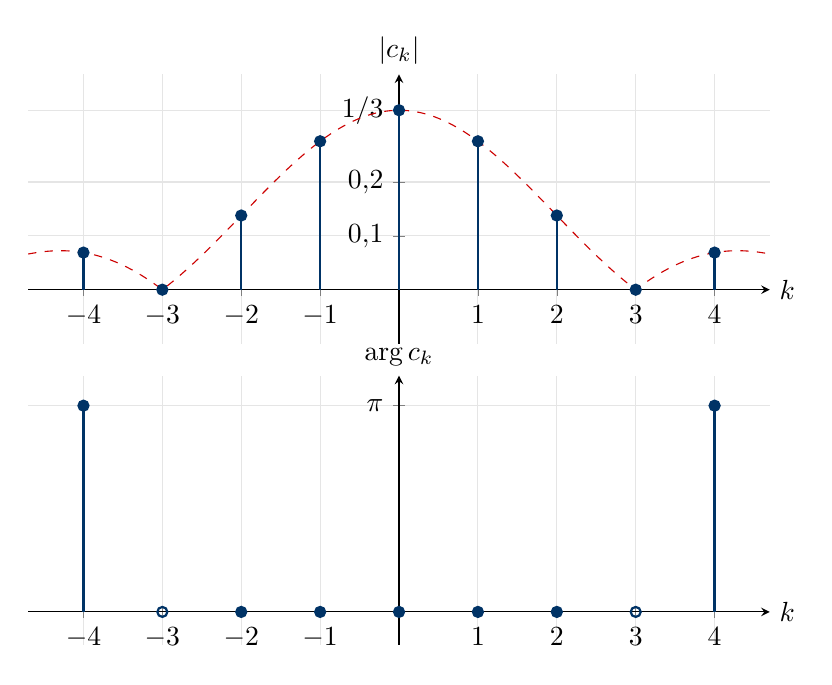
\begin{tikzpicture}

% --- Panel superior: módulo ---
\begin{axis}[
    name=modulo,
    width=11cm, height=5cm,
    xmin=-4.7, xmax=4.7,
    ymin=-0.10, ymax=0.40,
    xtick={-4,-3,-2,-1,0,1,2,3,4},
    ytick={0, 0.1, 0.2, 0.333},
    yticklabels={$0$, $0{,}1$, $0{,}2$, $1/3$},
    xlabel={$k$},
    ylabel={$|c_k|$},
    axis lines=middle,
    enlargelimits=false,
    grid=major,
    grid style={gray!20},
    every axis x label/.style={at={(ticklabel* cs:1)}, anchor=west},
    every axis y label/.style={at={(ticklabel* cs:1)}, anchor=south},
]
% Envolvente |sinc(k pi/3)/3| muestreada en muchos puntos
\addplot[utnred, dashed, samples=300, domain=-4.7:4.7]
    ({x}, {abs( (1/3) * sin(deg(x*pi/3))/(x*pi/3) )});
% Stems en k = -4..4
\addplot+[utnblue, thick, ycomb, mark=*, mark options={fill=utnblue, scale=0.9}]
    coordinates {
        (-4, 0.0689) (-3, 0) (-2, 0.1378) (-1, 0.2757) (0, 0.3333)
        (1, 0.2757) (2, 0.1378) (3, 0) (4, 0.0689)
    };
\end{axis}

% --- Panel inferior: fase ---
\begin{axis}[
    name=fase,
    at={(modulo.below south west)}, anchor=north west, yshift=-0.4cm,
    width=11cm, height=5cm,
    xmin=-4.7, xmax=4.7,
    ymin=-0.5, ymax=3.6,
    xtick={-4,-3,-2,-1,0,1,2,3,4},
    ytick={0, 3.1416},
    yticklabels={$0$, $\pi$},
    xlabel={$k$},
    ylabel={$\arg c_k$},
    axis lines=middle,
    enlargelimits=false,
    grid=major,
    grid style={gray!20},
    every axis x label/.style={at={(ticklabel* cs:1)}, anchor=west},
    every axis y label/.style={at={(ticklabel* cs:1)}, anchor=south},
]
% Fase: 0 para c_k>0, pi para c_k<0, indefinida en cruces
\addplot+[utnblue, thick, ycomb, mark=*, mark options={fill=utnblue, scale=0.9}]
    coordinates {(-4, 3.1416) (-2, 0) (-1, 0) (0, 0) (1, 0) (2, 0) (4, 3.1416)};
% k=3 y k=-3 con marcador hueco indicando indefinida
\addplot[utnblue, mark=o, mark options={scale=0.9, line width=0.8pt}, only marks]
    coordinates {(-3, 0) (3, 0)};
\end{axis}

\end{tikzpicture}
\end{document}
